\begin{abstract}

  \textbf{1. }
    Phylogenetic trees are currently routinely reconstructed from an alignment 
    of character sequences (usually nucleotide sequences). 
    Bayesian tools, such as MrBayes, RevBayes and BEAST2, 
    have gained much popularity over the last decade, 
    as they allow joint estimation of the posterior distribution of the 
    phylogenetic trees and the parameters of the underlying inference model.  
    An important ingredient of these Bayesian approaches is the species tree 
    prior.
    In principle, the Bayesian framework allows for comparing 
    different tree priors, which may elucidate the macroevolutionary 
    processes underlying the species tree.
    In practice, however, only macroevolutionary models that allow 
    for fast computation of the prior probability are used.
    The question is how accurate the tree estimation is when 
    the real macroevolutionary processes are substantially different 
    from those assumed in the tree prior. \\
    \textbf{2. }
    Here we present \verb;pirouette;, 
    a free and open-source R package that assesses 
    the inference error made by Bayesian phylogenetics 
    for a given macroevolutionary diversification model. 
    \verb;pirouette; makes use of 
    BEAST2, but its philosophy applies to any Bayesian phylogenetic inference 
    tool. \\
  \textbf{3. }
    We describe \verb;pirouette;'s usage \new{providing full examples in which 
    we interrogate a model for its power to describe another}. \\
  \textbf{4. }
    Last, we discuss the results obtained by the examples and their 
    interpretation. \\
\end{abstract}

{\bf Keywords:} Bayesian model selection, BEAST2, computational biology, evolution, phylogenetics, R, tree prior, babette

%%%%%%%%%%%%%%%%%%%%%%%%%%%%%%%%%%%%%%%%%%%%%%%%%%%%%%%%%%%%%%%%%%%%%%%%%%%%%%%%
\section{Introduction}
%%%%%%%%%%%%%%%%%%%%%%%%%%%%%%%%%%%%%%%%%%%%%%%%%%%%%%%%%%%%%%%%%%%%%%%%%%%%%%%%
\new{
	The development of new powerful Bayesian phylogenetic inference tools,
	such as BEAST [\cite{drummond2007beast}], 
	MrBayes [\cite{huelsenbeck2001mrbayes}]
	or RevBayes [\cite{hohna2016revbayes}] 
	has been a major advance in constructing phylogenetic trees 
	from character data (usually nucleotide sequences) extracted from organisms
	(usually extant, but extinction events and/or time-stamped data 
	can also be added), 
	and hence in our understanding of the main drivers 
	and modes of diversification.
}

\new{
	BEAST [\cite{drummond2007beast}] is a typical Bayesian phylogenetics tool, 
	that needs both character data and priors to infer 
	a posterior distribution of phylogenies.
	Specifically, for the species tree prior - which describes 
	the process of diversification - 
	BEAST has built-in priors such as the Yule [\cite{yule}] and 
	(constant-rate) birth-death (BD) [\cite{nee1994reconstructed}] models
	as well as coalescent priors.
	These simple tree priors are among the most commonly used, 
	as they represent some biologically realistic processes (e.g. 
	viewing diversification as a branching process), 
	while being computationally fast.
}

\new{
	To allow users to extend the functionalities of BEAST
	using plug-ins, BEAST2 was written [\cite{bouckaert2019beast}]
	(with BEAST and BEAST2 still independently being developed further).
	For example, one can add novel diversification models 
	by writing a BEAST2 plugin that contains 
	the likelihood formula of a phylogeny under the novel diversification model, 
	i.e. the prior probability of a species tree.
	Plugins have been provided, for instance, for the calibrated 
	Yule model [\cite{heled2015calibrated}],
	  the BD model with incomplete sampling [\cite{stadler2009incomplete}],
	  the BD model with serial sampling [\cite{stadler2012estimating}],
	  the BD serial skyline model [\cite{stadler2013birth}],
	  the fossilized BD process [\cite{gavryushkina2014bayesian}], and
	  the BD SIR model [\cite{kuhnert2014simultaneous}].
}

\new{
	Many other diversification models (and their associated likelihood algorithms) 
	have been developed, e.g., models in which diversification 
	is time-dependent [\cite{nee1994reconstructed,rabosky2008explosive}],
	or diversity-dependent [\cite{etienne2012diversity}],
	or where diversification rates change for specific lineages 
	and their descendants [\cite{etienne2012conceptual, rabosky2014automatic, alfaro2009nine, laudanno2020detecting}].
	Other models treat speciation as a process that takes 
	time [\cite{rosindell2010protracted, etienne2012prolonging, lambert2015reconstructed}],
	or where diversification rates
	depends on one or more traits 
	[\cite{maddison2007estimating, fitzjohn2012diversitree, herrera2019detecting}].
}

\new{
	These are, however, not yet available as tree priors in BEAST2, 
	for reasons explained below. In this paper, 
	we present methodology to determine whether such new plug-ins are needed, 
	or whether currently available plug-ins are sufficient. 
	We show this using the Yule and BD species tree priors, 
	but our methods can be used with other built-in tree priors as well.
}

\new{
	The rationale of our paper is as follows. 
}
When a novel diversification model is introduced,
its performance in inference should be tested.
Part of a model's performance is its ability to 
recover parameters from simulated data with known 
parameters (e.g. [\cite{etienne2014estimating}]), 
where ideally the estimated parameter values closely match the known/true values.
Even when a diversification model passes this test, 
it is not necessarily used as tree prior in Bayesian inference.
Bayesian phylogenetic inference often requires 
that the prior probability of the phylogeny 
according to the diversification model has to be computed millions of times. 
Therefore, biologically interesting but computationally expensive tree priors 
are often not implemented, and simpler priors are used instead. 
This is not necessarily problematic, when the data are very informative 
\new{
  or when the prior is truly uninformative
}, 
as this will reduce the influence of the tree prior.
However, the assumption that tree prior choice is of low \new{impact} 
must first be verified.

There have been multiple attempts to investigate the \new{impact} of tree
prior choice. For example, Sarver and colleagues, [\cite{sarver2019choice}] 
showed that the choice of tree prior does not 
substantially affect phylogenetic inferences of diversification rates.
However, they only compared current diversification models to one another, 
and thus this does not inform us on the \new{impact} of a new tree prior.

\new{
Similarly,
Ritchie and colleagues [\cite{Ritchie2017impact}] showed that inference was accurate when birth-death or skyline coalescent priors were used, but they simulated their trees with a Yule process only, as their focus was not so much on the diversification process but on the influence of inter- and intraspecific sampling.
}

\new{Another way to benchmark a diversification model, is by doing a model comparison, in which the best model is determined
from a set of models. A good early example is \citet{goldman1993statistical} 
in which Goldman compared DNA substitution models.
A recent approach to test the impact of tree prior choice, proposed
by \citet{duchene2018phylodynamic}, allows to measure
model adequacy for phylodynamic models that are
mathematically described (i.e. have a known likelihood equation).}

Here we introduce a method to quantify the \new{impact} 
of a novel tree prior,
\new{
  i.e., a tree model, for which we can simulate phylogenies, but not yet
  calculate their likelihoods.
}
\new{This new method simultaneously assesses the substitution, clock and tree models [\cite{duchene2015evaluating}].}
The method starts with a phylogeny generated by the new model. 
Next, nucleotide sequences are simulated that follow the evolutionary 
history of the given phylogeny. 
Then, using BEAST2's built-in tree priors,
a Bayesian posterior distribution of phylogenies is inferred. 
We then compare the inferred with the original phylogenies. 
How to properly perform this comparison forms the heart of our method.
Only new diversification models that result 
in a large discrepancy between inferred and simulated phylogenies 
will be worth the effort and computational burden to implement 
a species tree prior for in a Bayesian framework.

Our method is programmed as an R package [\cite{R}] called \verb;pirouette;.
\verb;pirouette; is built on \verb;babette; [\cite{bilderbeek2018babette}], 
which calls BEAST2 [\cite{bouckaert2019beast}]. 

%%%%%%%%%%%%%%%%%%%%%%%%%%%%%%%%%%%%%%%%%%%%%%%%%%%%%%%%%%%%%%%%%%%%%%%%%%%%%%%%
\section{Description}
%%%%%%%%%%%%%%%%%%%%%%%%%%%%%%%%%%%%%%%%%%%%%%%%%%%%%%%%%%%%%%%%%%%%%%%%%%%%%%%%

The goal of \verb;pirouette; is to quantify the \new{impact of a new} tree prior.
It does so by measuring the inference error made 
for a given reconstructed phylogeny, 
simulated under a (usually novel) diversification model.
We refer to the model that has generated the given tree 
as the 'generative tree model' $\mathit{p_{G}}$.
\new{
  A 'generative tree model', in this paper, can be either the novel diversification model for which we are testing the impact of choosing standard tree priors for, or it is the model with which we generate the twin tree that is needed for comparison (see below). In the latter case, we also refer to it as the actual generative tree model, and it thus serves as a baseline model. This is is done in the example, where the Yule model is the generative model.
}

\new{
  The inference error we aim to quantify is not of stochastic nature.
  Stochastic errors are usually non-directional.
  We, instead, aim to expose the bias due to the mismatch between 
  a generative model (that has generated the phylogeny) and the model(s) used in the actual inference.
}
We define the birth-death \new{(BD)} model [\cite{nee1994reconstructed}] as
the standard tree model, as many (non-standard) tree models 
have a parameter setting \new{such that it reduces} to this model. 
One such example is the diversity-dependent (DD) diversification 
model [\cite{DDD, etienne2012diversity}] in which speciation 
or extinction rate depends 
on the number of species and a clade-level carrying capacity.
\new{
  The BD model can be seen as a special case of the DD model, because for
} 
an infinite carrying capacity, the DD model reduces to the BD model.
When benchmarking a novel tree model, 
one will typically construct phylogenies 
for different combinations of the diversification model's parameters, 
to assess under which scenarios the inference error cannot be neglected. 
While we recommend many replicate simulations 
when assessing a novel tree prior, 
our example contains only one replicate,
as the goal is to show the workings of \verb;pirouette;,
instead of doing an extensive analysis.
The supplementary material includes results of replicated runs under multiple settings.

\verb;pirouette; allows the user to specify a wide variety of custom settings. 
These settings can be grouped in macro-sections, 
according to how they operate in the pipeline. 
We summarize them in Table~\ref{tab:options} and Table~\ref{tab:definitions}.

\begin{sidewaystable}
\centering
  \begin{tabular}{|p{3.4cm}|p{9.7cm}|p{4.5cm}@{}|}
    \hline
    \centering
    %%%%%%%%%%%%%%%%%%%%%%%%%%%%%%%%%%%%%%%%%%%%%%%%%%%%%%%%%%%%%%%%%%%%%%%%%%%%
    \textbf{Sub-argument} & 
    \textbf{Description} &
    \textbf{Possible values} \\ 
    \hline
    %%%%%%%%%%%%%%%%%%%%%%%%%%%%%%%%%%%%%%%%%%%%%%%%%%%%%%%%%%%%%%%%%%%%%%%%%%%%
    \verb;tree_prior; &
    Macroevolutionary diversification model &
    BD, CBS, CCP, CEP, Yule \\
    %%%%%%%%%%%%%%%%%%%%%%%%%%%%%%%%%%%%%%%%%%%%%%%%%%%%%%%%%%%%%%%%%%%%%%%%%%%%
    \verb;clock_model; &
    Clock for the DNA mutation rates &
    RLN, strict \\
    %%%%%%%%%%%%%%%%%%%%%%%%%%%%%%%%%%%%%%%%%%%%%%%%%%%%%%%%%%%%%%%%%%%%%%%%%%%%
    \verb;site_model; &
    Nucleotide substitution model &
    GTR, HKY, JC, TN \\
    %%%%%%%%%%%%%%%%%%%%%%%%%%%%%%%%%%%%%%%%%%%%%%%%%%%%%%%%%%%%%%%%%%%%%%%%%%%%
    \verb;mutation_rate; &
    Pace at which \new{substitutions occur} &
    \verb;mutation_rate; $\in \mathbb{R}_{>0}$\\
    %%%%%%%%%%%%%%%%%%%%%%%%%%%%%%%%%%%%%%%%%%%%%%%%%%%%%%%%%%%%%%%%%%%%%%%%%%%%
    \verb;root_sequence; &
    DNA sequence at the root of the tree &
    any combination of a, c, g, t \\
    %%%%%%%%%%%%%%%%%%%%%%%%%%%%%%%%%%%%%%%%%%%%%%%%%%%%%%%%%%%%%%%%%%%%%%%%%%%%
    \verb;model_type; &
    Criterion to select an inference model &
    Generative, Candidate \\
    %%%%%%%%%%%%%%%%%%%%%%%%%%%%%%%%%%%%%%%%%%%%%%%%%%%%%%%%%%%%%%%%%%%%%%%%%%%%
    \verb;run_if; &
    Condition under which an inference model is used &
    Always, Best candidate \\
    %%%%%%%%%%%%%%%%%%%%%%%%%%%%%%%%%%%%%%%%%%%%%%%%%%%%%%%%%%%%%%%%%%%%%%%%%%%%
    \verb;do_measure_evidence; &
    Sets whether or not the evidence of the model must be computed &
    TRUE, FALSE \\
    %%%%%%%%%%%%%%%%%%%%%%%%%%%%%%%%%%%%%%%%%%%%%%%%%%%%%%%%%%%%%%%%%%%%%%%%%%%%
    \verb;error_fun; &
    Specifies how to measure the error &
    nLTT, $|\gamma|$ \\
    %%%%%%%%%%%%%%%%%%%%%%%%%%%%%%%%%%%%%%%%%%%%%%%%%%%%%%%%%%%%%%%%%%%%%%%%%%%%
    \verb;burn_in_fraction; &
    Specifies the percentage of initial posterior trees to discard &
    \verb;burn_in_fraction; $\in [0, 1]$\\
    %%%%%%%%%%%%%%%%%%%%%%%%%%%%%%%%%%%%%%%%%%%%%%%%%%%%%%%%%%%%%%%%%%%%%%%%%%%%
    \hline
  \end{tabular}
  \caption{
    Most important parameter options.
    BD = birth death [\cite{nee1994reconstructed}], 
    CBS = coalescent Bayesian skyline [\cite{drummond2005bayesian}], 
    CCP = coalescent constant-population, 
    CEP = coalescent exponential-population,
    Yule = pure birth model [\cite{yule}],
    RLN = relaxed log-normal clock model [\cite{drummond2006relaxed}],
    strict = strict clock model [\cite{zuckerkandl1965molecules}], 
    GTR = Generalized time-reversible model [\cite{tavare1986some}], 
    HKY = Hasegawa, Kishino and Yano [\cite{hasegawa1985dating}], 
    JC = Jukes and Cantor [\cite{jukes1969evolution}], 
    TN = Tamura and Nei [\cite{tamura1993estimation}],
    nLTT = normalized lineages-through-time [\cite{janzen2015approximate}],
    $|\gamma|$ = absolute value of the gamma statistic [\cite{pybus2000testing}].
  }
  \label{tab:options}
\bigskip

  \begin{tabular}{|@{}c|p{4cm}|p{12.2cm}|}
    \hline
    \centering
    %%%%%%%%%%%%%%%%%%%%%%%%%%%%%%%%%%%%%%%%%%%%%%%%%%%%%%%%%%%%%%%%%%%%%%%%%%%%
    \textbf{Symbol} &
    \textbf{Macro-argument} &
    \textbf{Description} \\
    \hline
    %%%%%%%%%%%%%%%%%%%%%%%%%%%%%%%%%%%%%%%%%%%%%%%%%%%%%%%%%%%%%%%%%%%%%%%%%%%%
    $\mathit{G}$ &
    Generative model &
    The full setting to produce BEAST2 input data. 
    Its core features are the tree prior $\mathit{p_{G}}$, the clock 
    model $\mathit{c_{G}}$ and the site model $\mathit{s_{G}}$. \\
    %%%%%%%%%%%%%%%%%%%%%%%%%%%%%%%%%%%%%%%%%%%%%%%%%%%%%%%%%%%%%%%%%%%%%%%%%%%%  
    $\mathit{s_{G}}$ &
    Site model &
    Both the substitution model and rate variation across sites. \\
    %%%%%%%%%%%%%%%%%%%%%%%%%%%%%%%%%%%%%%%%%%%%%%%%%%%%%%%%%%%%%%%%%%%%%%%%%%%%
    $\mathit{A}$ &
    Alignment model &
    Specifies the alignment generation, such as the clock model 
    $\mathit{c_{G}}$, site model $\mathit{s_{G}}$ and root sequence. \\
    %%%%%%%%%%%%%%%%%%%%%%%%%%%%%%%%%%%%%%%%%%%%%%%%%%%%%%%%%%%%%%%%%%%%%%%%%%%%
    $\mathit{X_{i}}$ &
    $i$-th candidate experiment &
    Full setting for a Bayesian inference. It is made by a 
    candidate inference model $\mathit{I_{i}}$ and its 
    inference conditions $\mathit{C_{i}}$. \\
    %%%%%%%%%%%%%%%%%%%%%%%%%%%%%%%%%%%%%%%%%%%%%%%%%%%%%%%%%%%%%%%%%%%%%%%%%%%%
    $\mathit{I}$ &
    Inference model &
    The assumed phylogenetic inference model, of which the main components
    are the tree prior $\mathit{p_{I}}$, assumed clock model $\mathit{c_{I}}$ 
    and assumed site model $\mathit{s_{I}}$. \\
    %%%%%%%%%%%%%%%%%%%%%%%%%%%%%%%%%%%%%%%%%%%%%%%%%%%%%%%%%%%%%%%%%%%%%%%%%%%%
    $\mathit{C}$ & Inference conditions & Conditions under which $\mathit{I}$ 
    is used in the inference. 
    They are composed of the model type, run condition and 
    whether to measure the evidence. \\
    %%%%%%%%%%%%%%%%%%%%%%%%%%%%%%%%%%%%%%%%%%%%%%%%%%%%%%%%%%%%%%%%%%%%%%%%%%%%
    $\mathit{E}$ & Error measure parameters & 
    Errors measurement setup that can be specified providing an 
    error function to measure the difference between the original phylogeny 
    and the inferred posterior. The first iterations of the MCMC chain of the 
    posterior may not be representative and can be discarded using a burn-in 
    fraction. \\
    %%%%%%%%%%%%%%%%%%%%%%%%%%%%%%%%%%%%%%%%%%%%%%%%%%%%%%%%%%%%%%%%%%%%%%%%%%%%
    \hline 
  \end{tabular}
  \caption{
    Definitions of terms and relative symbols used in the main text and in 
    Fig~\ref{fig:pipeline}. To run the pipeline $\mathit{A}$, $\mathit{X}$ 
    and $\mathit{E}$ must be specified.
  }
  \label{tab:definitions}
\end{sidewaystable}

\subsection{pirouette's pipeline}
\label{subsec:pipeline}

\begin{figure}
  \centering
  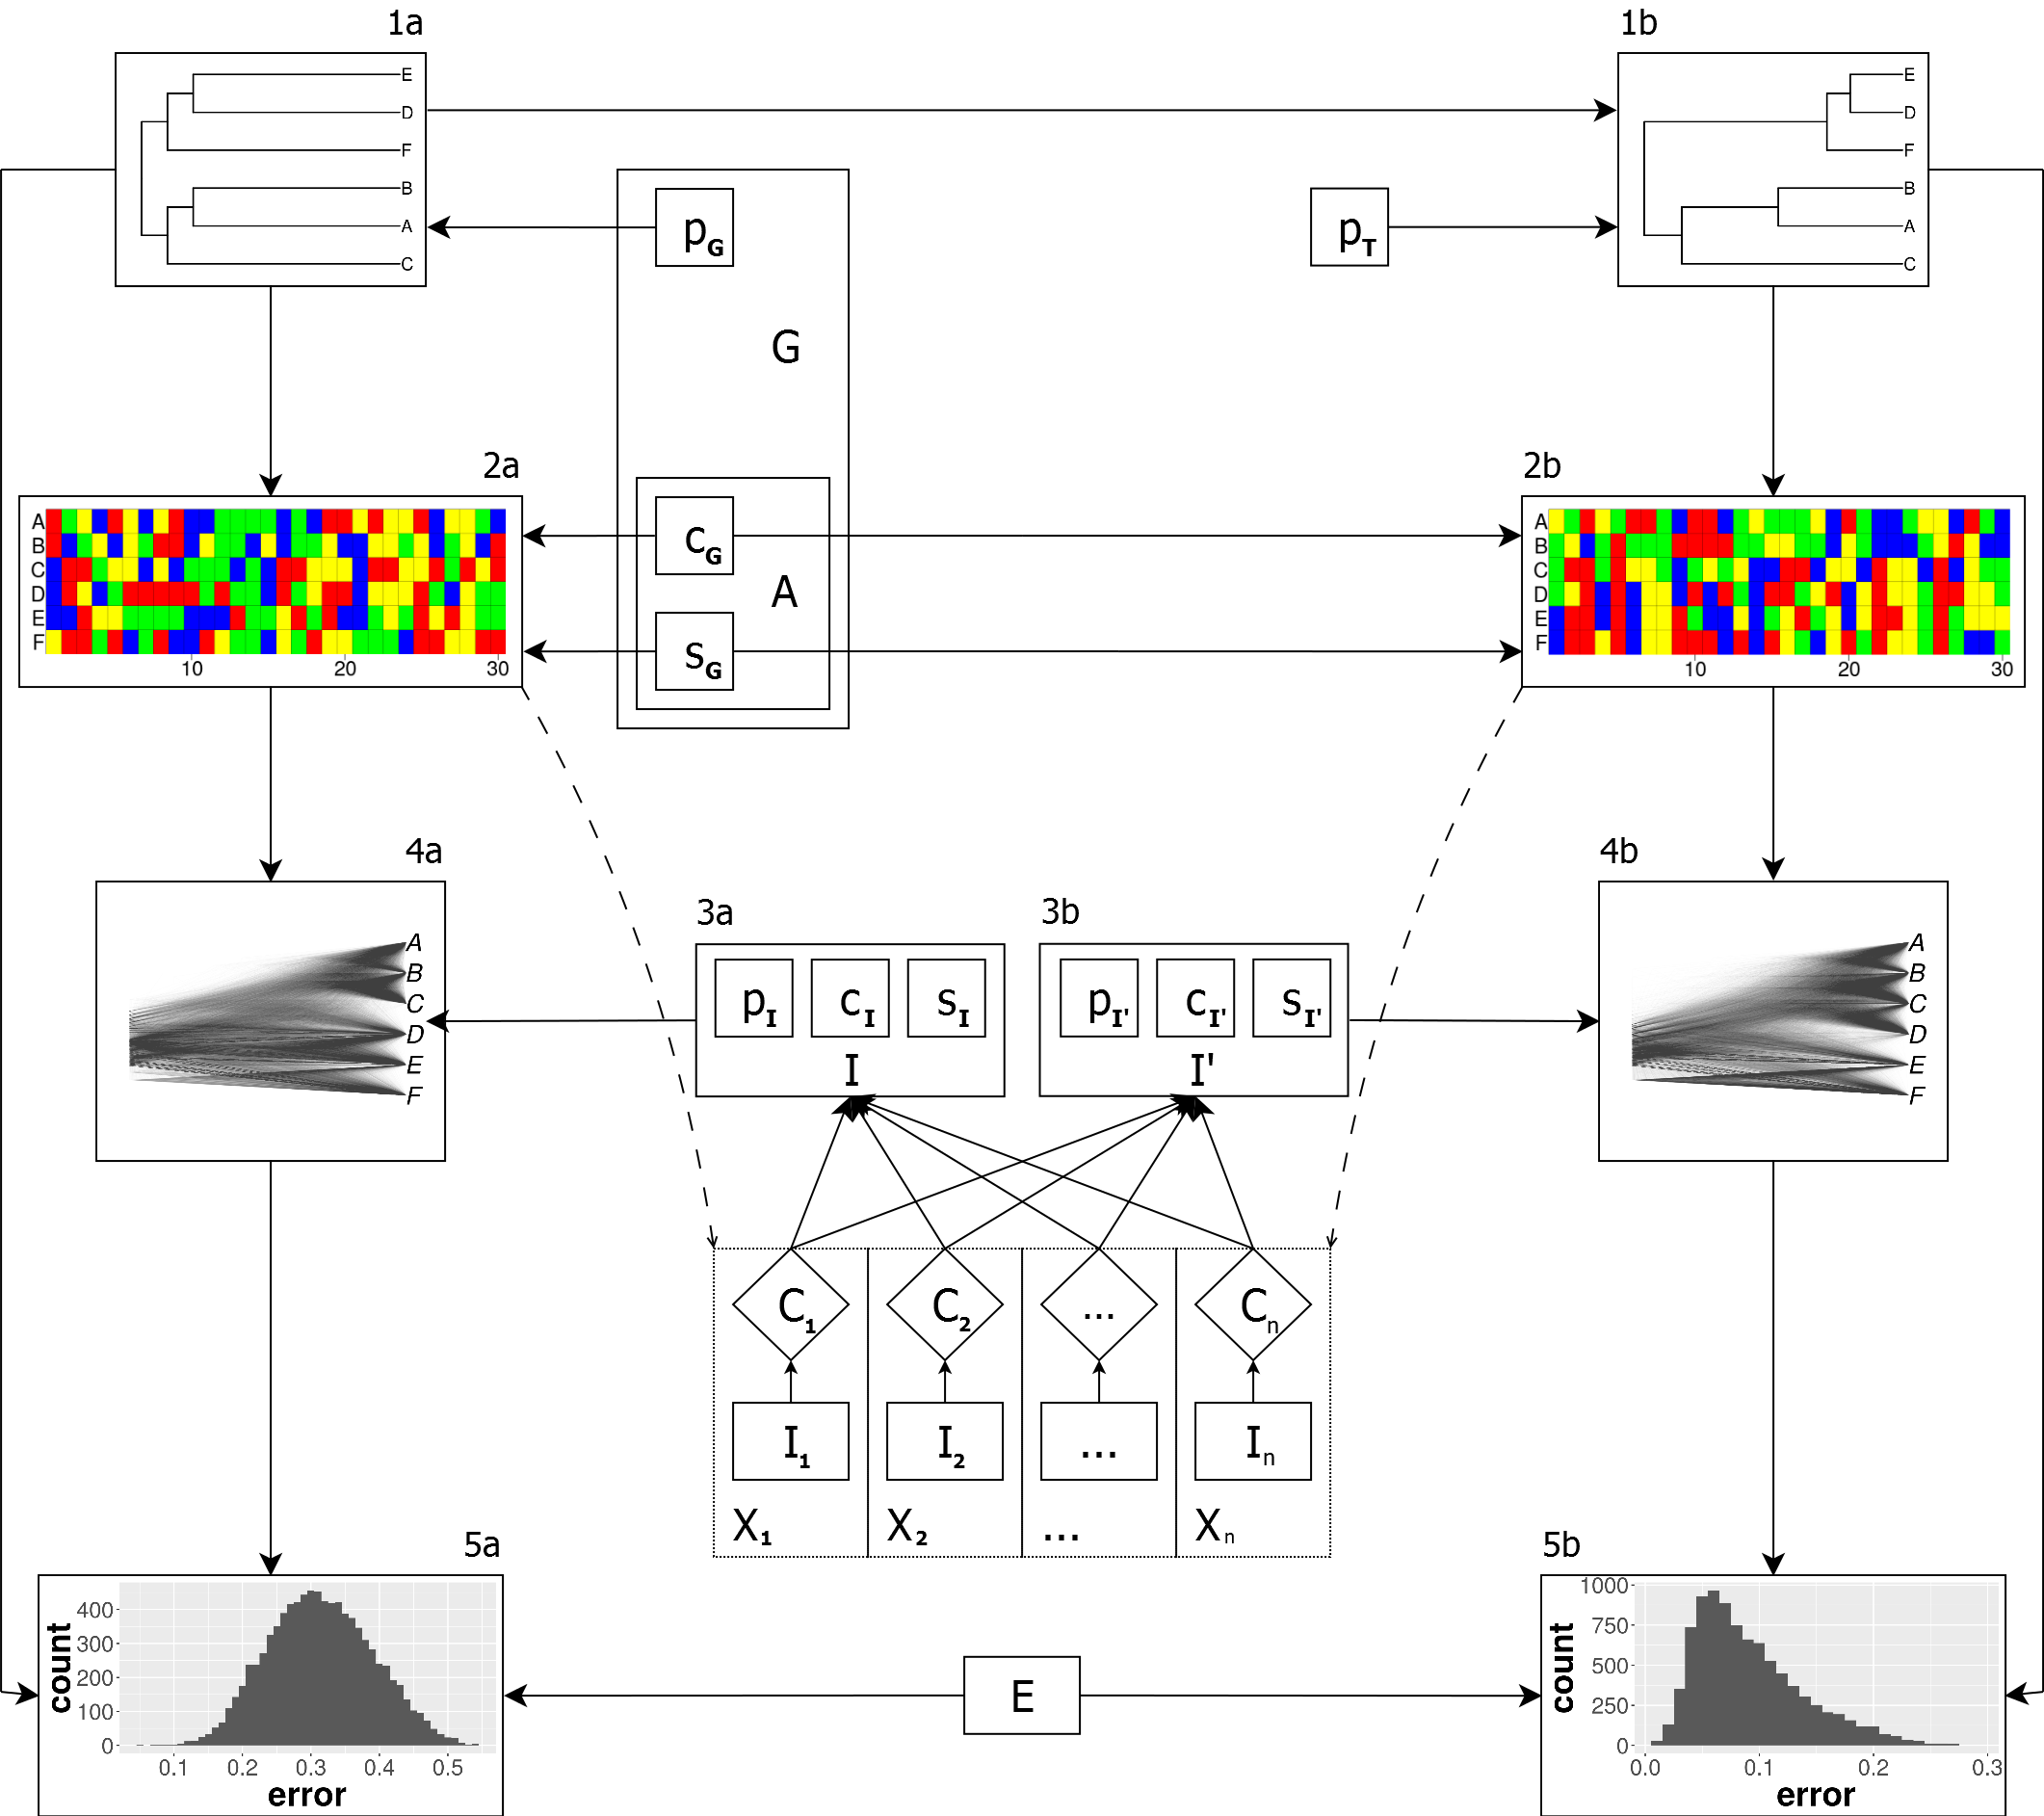
\includegraphics[width = 0.97\textwidth]{workflow4.png}
  \caption{
    \texttt{pirouette} pipeline.
    The pipeline starts from a phylogeny (1a) simulated by the 
    generative tree model 
    $\mathit{p_{G}}$.
    The phylogeny is converted to an alignment (2a) using the generative 
    alignment model 
    $\mathit{A} = (\mathit{c_{G}}, \mathit{s_{G}})$, composed of a clock model 
    and a site model. 
    The user defines one or more experiments.
    For each candidate experiment $\mathit{X_{i}}$ 
    (a combination of inference model $\mathit{I_{i}}$ and condition $\mathit{C_{i}}$),
    if its condition $\mathit{C_{i}}$ is 
    satisfied (which can depend on the alignment), 
    the corresponding inference model $\mathit{I} = \mathit{I_{i}}$ is selected
    to be used in the next step.
    The inference models (3a) of the selected experiments use the alignment (2a) 
    to each create a Bayesian posterior of (parameter estimates and) 
    phylogenies (4a). 
    Each of the posterior trees is compared to the true phylogeny (1a) 
    using the error measure $\mathit{E}$, 
    resulting in an error distribution (5a). 
    Optionally, for each selected inference model a twin pipeline can be run.
    A twin phylogeny (1b) can be generated from the original 
    phylogeny (1a) using the twin tree model $\mathit{p_{t}}$, 
    selected among standard diversification models; 
    the default option is the standard BD model, 
    with parameters estimated from the original phylogeny.
    A twin alignment (2b) is then simulated from the twin phylogeny 
    using clock model $\mathit{c_{G}}$ and site model $\mathit{s_{G}}$ 
    used with the generative tree model (the novel tree model).
    The twin pipeline follows the procedure of the main pipeline, 
    resulting in a twin error distribution (5b).
  }
  \label{fig:pipeline}
\end{figure}

The pipeline to assess the error BEAST2 makes in inferring this phylogeny 
contains the following steps:
\begin{enumerate}
  \item The user supplies one or (ideally) more phylogenies from a 
    new diversification model.
  \item From the given phylogeny an alignment is simulated 
    under a known alignment model $\mathit{A}$.
  \item From this alignment, according to the specified 
    inference conditions $\mathit{C}$, 
    an inference model $\mathit{I}$ is chosen (which may or may not differ 
    from the model that generated the tree).
  \item The inference model and the alignment are used 
    to infer a posterior distribution of phylogenies.
  \item The phylogenies in the posterior are compared with the given phylogeny 
    to estimate the error made, according to 
    the error measure $\mathit{E}$ specified by the user.
\end{enumerate}

The pipeline is visualized in Fig.~\ref{fig:pipeline}. 
There is also the option to generate a 'twin tree', 
that goes through the same pipeline (see supplementary subsection \ref{subsec:twinning}). 

The first step simulates an alignment from the given 
phylogeny (Fig.~\ref{fig:pipeline}, 1a $\rightarrow$ 2a).
For the sake of clarity, here we will assume the alignment consists
of DNA sequences, but one can also use other heritable materials such as amino acids.
The user must specify a root sequence (i.e. the DNA sequence of the shared 
common ancestor of all species), a mutation rate and a site model.

The second step (Fig.~\ref{fig:pipeline}, 3a)
selects one or more inference model(s) $I$ from 
a set of standard inference models $I_{1},\dots,I_{n}$.
For example, if the generative model is known and standard (which it is for the twin tree, see below),
one can specify the inference model to be the same as the generative model.
If the tree model is unknown or non-standard - which is the primary 
motivation for this paper -, one can pick
a standard inference model which is considered 
to be closest to the true tree model.
Alternatively, if we want to run only the inference
model that fits best to an alignment from a set of candidates \new{(regardless of whether these generated the alignments)},
one can specify these inference models (see section \ref{subsec:candidates}).

The third step infers the posterior distributions,
using the simulated alignment (Fig.~\ref{fig:pipeline}, 2a $\rightarrow$ 4a),
and the inference models that were selected in the previous step (3a). 
For each selected experiment a posterior distribution is inferred, using the 
\verb;babette; [\cite{bilderbeek2018babette}] R package which makes use of BEAST2. 

The fourth step quantifies the new{impact of choosing standard models for inference, i.e.} the inference error made. 
First the burn-in fraction is removed, i.e. the first phase of the 
Markov chain Monte Carlo (MCMC) run,
which samples an unrepresentative part of parameter and tree space. 
From the remaining posterior, \verb;pirouette; 
creates an error distribution, by measuring the difference
between the true tree and each of the posterior 
trees (Fig.~\ref{fig:pipeline}, 4a $\rightarrow$ 5a).
The user can specify a function to quantify the differences between
the true and posterior trees. 

\subsection{Controls}\label{subsec:controls}

\verb;pirouette; allows for
two types of control measurements. The first type of control
is called 'twinning', which results in an error distribution
that is the baseline error of the inference pipeline (see
supplementary materials, subsection \ref{subsec:twinning} for more details). \new{This the error that arises when the models used in inference are identical to the ones used in generating the alignments.}
The second type of control is the use of candidate models,
which result in an error distribution
for a generative model that is determined to be the best fit to
the tree (see supplementary materials, 
section \ref{subsec:candidates} for more details). \new{The underlying idea is that using a substitution model in inference than used in generating the alignment may partly compensate for choosing a standard tree model instead of the generative tree model as tree prior in inference.}
Additionally, multiple \verb;pirouette; runs are needed
to reduce the influence of stochasticity (see supplementary materials, 
section \ref{subsec:stochasticity} for more details).

%%%%%%%%%%%%%%%%%%%%%%%%%%%%%%%%%%%%%%%%%%%%%%%%%%%%%%%%%%%%%%%%%%%%%%%%%%%%%%%%
\section{Usage}
%%%%%%%%%%%%%%%%%%%%%%%%%%%%%%%%%%%%%%%%%%%%%%%%%%%%%%%%%%%%%%%%%%%%%%%%%%%%%%%%

We show the usage of \verb;pirouette; on a tree generated 
by the non-standard diversity-dependent (DD) tree 
model [\citep{DDD, etienne2012diversity}],
which is a BD model with a speciation rate that depends on the number of species. 

The code to reproduce our results can be found at  
\url{https://github.com/richelbilderbeek/pirouette_example_30}
and a simplified version is shown here for convenience:

\begin{lstlisting}[language=R]
library(pirouette)

# Create a DD phylogeny with 6 taxa and a crown age of 10
phylogeny <- create_exemplary_dd_tree()

# Use standard pirouette setup. This creates a list object with all settings for generating the alignment, the inference using BEAST2, the twinning parameters to generate the twin tree and infer it using BEAST2, and the error measure  
pir_params <- create_std_pir_params()

# Do the runs
pir_out <- pir_run(
  phylogeny = phylogeny,
  pir_params = pir_params
)

# Plot
pir_plot(pir_out)
\end{lstlisting}

The DD tree generated by this code is shown in Figure \ref{fig:dd_tree}. 

\begin{figure}[H]
  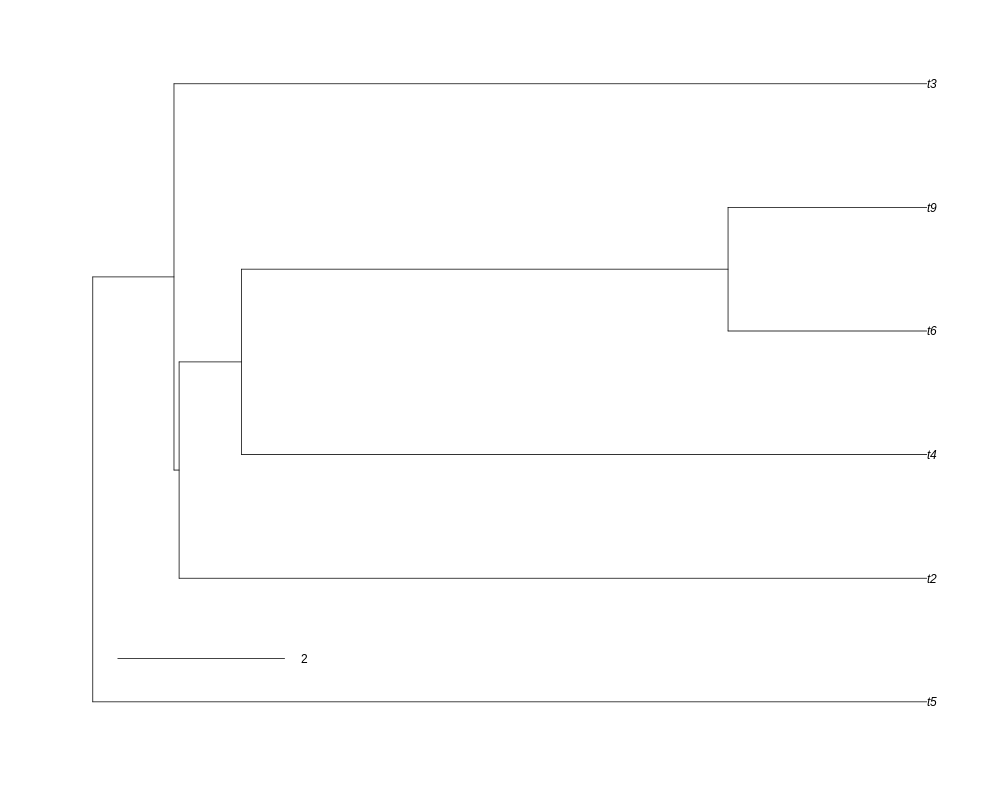
\includegraphics[width=\textwidth]{pirouette_example_30/example_30/true_tree.png}
  \caption{
    The example tree resulting from a diversity-dependent (DD) simulation.
  }
  \label{fig:dd_tree}
\end{figure}

The error distribution shown in Figure \ref{fig:example_30}
is produced, which uses the nLTT statistic [\cite{janzen2015approximate}] to compare phylogenies (see 
section \ref{subsec:nltt} for details regarding the nLTT statistic
and its caveats).

\begin{figure}[H]
  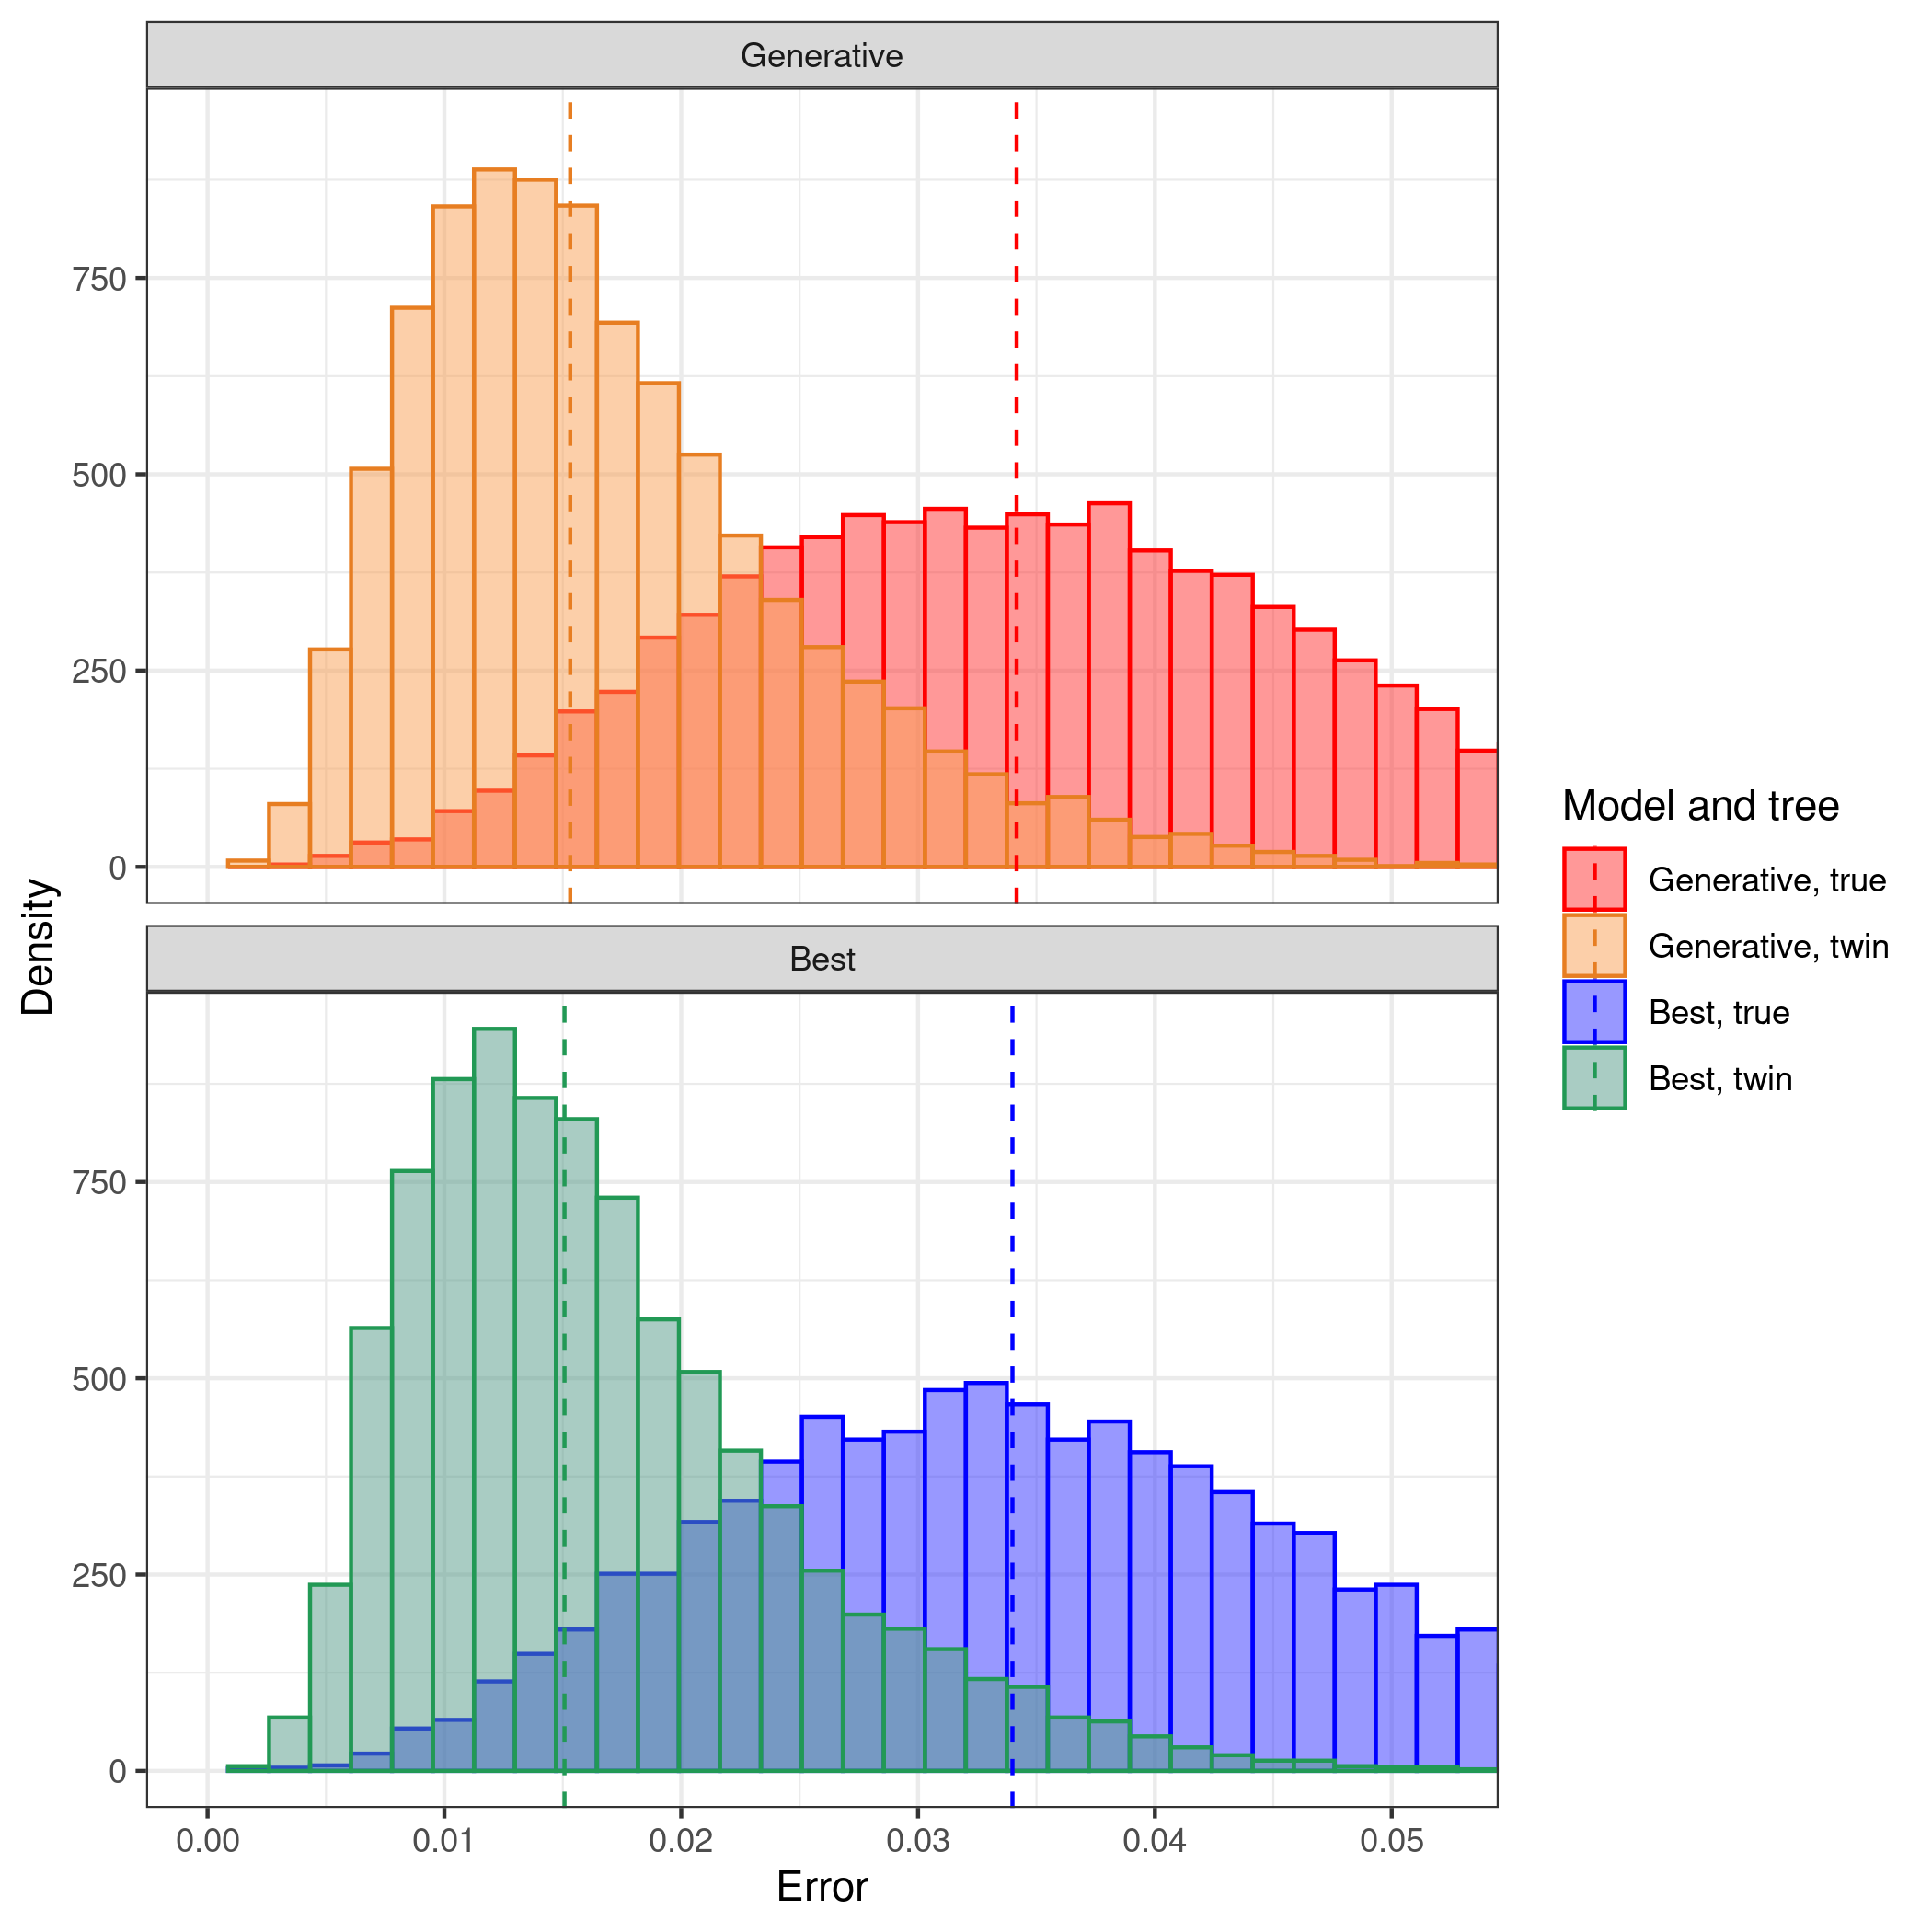
\includegraphics[width=0.9\textwidth]{pirouette_example_30/errors.png}
  \caption{
    \new{
      The impact of the tree prior for 
      the example tree in Figure \ref{fig:dd_tree}. 
      The alignment for this true tree was generated using a JC substitution model 
      and strict clock model. 
      For inferring the tree from this alignment in the 'generative' scenario 
      the same substitution and clock models were used, 
      and a Yule tree prior (this is the assumed generative model,
      because the real generative model is of course unknown). 
      In the 'best' scenario the best-fitting candidate 
      models (TN substitution model, strict clock model and Yule tree prior) 
      were used. For the twin tree, the same models were chosen, 
      except that BD was used to generate and infer the twin tree.
      The twin distributions show the baseline inference error.
    }
    Vertical dashed lines show the median error value per distribution.
  }
  \label{fig:example_30}
\end{figure}

In the upper panel of Figure \ref{fig:example_30},
we can see that the error distributions of the \new{ (assumed) generative model (i.e. the known generative substitution and clock models, and the tree model that is assumed in inference of the true tree, and the tree model that is used for generating and inferring the twin tree)}
differ strongly between the true and twin tree. 
This difference shows the extent of the mismatch between
the true tree model (which is DD) and the (Yule) tree prior used in inference.
Because these distributions are distinctively different,
the inference error made when using an 
incorrect tree prior on a DD tree is profound.

Comparing the upper and lower panel of Figure \ref{fig:example_30}, 
we can see that the best
candidate model is only slightly better at inferring the true tree,
than the (assumed) generative model, 
thereby showing that they cannot compensate 
for the true generative tree model not being among the inference models.

The candidate model that had highest evidence given the simulated alignment,
was TN, strict and BD (see Table \ref{tab:options} for the meaning of these 
abbreviations). 
The TN site model is a surprising result: it assumes nucleotide substitutions 
occur at different rates between translations and transversions 
and that nucleotides are available with different frequencies (that is,
a nucleotide may be rare or overabundant).
The strict clock model matches the model how the alignment is simulated.
\new{
  The Yule model is not surprising as it is the standard tree prior 
  that is probably closest to the true DD model because it shows 
  no pull-of-the-present (but also no slowdown).
}

%%%%%%%%%%%%%%%%%%%%%%%%%%%%%%%%%%%%%%%%%%%%%%%%%%%%%%%%%%%%%%%%%%%%%%%%%%%%%%%%
\section{Discussion}
%%%%%%%%%%%%%%%%%%%%%%%%%%%%%%%%%%%%%%%%%%%%%%%%%%%%%%%%%%%%%%%%%%%%%%%%%%%%%%%%

We showed how to use \verb;pirouette; to quantify the \new{impact of a 
tree prior in Bayesian phylogenetics, assuming - for illustrative purposes - the simplest standard substitution, clock and
tree models, but also the models that would be selected among many different standard tree priors according to the highest marginal likelihood, as this would be a likely strategy for an empiricist. We recommend exploring different candidate models, but note that this is computationally highly demanding.}

Figure~\ref{fig:example_30} illustrates the primary result of our pipeline: 
it shows the error distributions for the true tree and the twin tree \new{
when either the generative model (for substitution and clock models these are known, for the tree model it must be assumed for the true tree and it is known for the twin tree) or the best-fitting set candidate model (i.e. combination of tree model, substitution model and clock model) is used in inference.} 
The clear difference between the error distributions 
for the true tree and the twin tree suggests 
that the choice of tree prior matters.
We note, however, that only one tree from a novel tree model
is not enough to determine the \new{impact} of using an incorrect
tree prior. Instead, a distribution 
of multiple trees, generated by the novel tree model, should be used. In the supplementary material we have provided some examples.

Like most phylogenetic experiments, the setup of \verb;pirouette;
involves many choices. A prime example is the
length of the simulated DNA sequence. One expects that the inference error
decreases for longer DNA sequences. We investigated this
superficially and confirmed this prediction (see the supplementary material). 
However, we note that for longer DNA sequences, the assumption 
of the same substitution rates across the entire sequence may become less realistic (different genes may experience different substitution rates)
and hence longer sequences may require more parameters. 
Hence, simply getting longer sequences will not always lead to a drastic 
reduction of the influence of the species tree prior.
Fortunately, \verb;pirouette; provides a pipeline that works for all choices.

Interpreting the results of \verb;pirouette; is up to the user; 
\verb;pirouette; does not answer the question 
whether the inference error is too large to trust the inferred tree. The user is encouraged to use different statistics to measure the error. The nLTT statistic is
a promising starting point, as it can compare any two trees and 
results in an error distribution of known range, but one may also explore other statistics.
In principle, \verb;pirouette; allows for this, but in our example we used a diversification model (DD) that only deviates from the Yule and BD models in the temporal branching pattern, not in the topology.
\new{
  For models that make different predictions on topology, 
  the twinning process should be modified.
}
\new{
	As noted in the introduction, Duch\^{e}ne and 
	colleagues [\cite{duchene2018phylodynamic}]
	also developed a method to assess the adequacy of a tree model
	on empirical trees. They simulated trees from the posterior distribution of 
	the parameters and then compared this to the originally inferred tree using 
	tree statistics, to determine whether the assumed tree model in inference 
	indeed generates the tree as inferred. This is useful if these trees match, 
	but when they do not, this does not mean that the inferred tree is incorrect; 
	if sufficient data is available the species tree prior may not be important,
	and hence inference may be adequate 
	even though the assumed species tree prior is not. 
	In short, the approach is applied to empirical trees and 
	compares the posterior and prior distribution of trees (with the latter 
	generated with the posterior parameters!).
    By contrast,}
    \verb;pirouette;
	\new{aims to expose when assuming standard priors for the 
	species tree are a mis- or underparameterization. 
	Hence, our approach applies to simulated trees and compares 
	the posterior distributions of trees generated with 
	a standard and non-standard model, but inferred with a standard one. 
	The two methods therefore complement one another.
}
Furthermore, we note that the \verb;pirouette; pipeline is not restricted 
to exploring the effects of a new species tree model. 
The pipeline can also be used to explore the effects of non-standard 
clock or site models, such as relaxed clock models with a non-standard 
distribution, correlated substitutions on sister lineages, or elevated 
substitutions rates during speciation events. 
It is, however, beyond the scope of this paper to discuss all these options 
in more detail.

In conclusion, \verb;pirouette; can show the errors to be expected
when the model assumed in inference is different from the actual generative model.
The user can then judge whether or not this new model 
should be implemented in the Bayesian phylogenetic tool. 

%%%%%%%%%%%%%%%%%%%%%%%%%%%%%%%%%%%%%%%%%%%%%%%%%%%%%%%%%%%%%%%%%%%%%%%%%%%%%%%%
% Bibliography
%%%%%%%%%%%%%%%%%%%%%%%%%%%%%%%%%%%%%%%%%%%%%%%%%%%%%%%%%%%%%%%%%%%%%%%%%%%%%%%%
% MEE style
\bibliographystyle{pirouette_mee}
\bibliography{pirouette_article}
%%%%%%%%%%%%%%%%%%%%%%%%%%%%%%%%%%%%%%%%%%%%%%%%%%%%%%%%%%%%%%%%%%%%%%%%%%%%%%%%

